\documentclass{beamer}
\mode<presentation>
\usepackage{amsmath,amssymb,mathtools}
\usepackage{textcomp}
\usepackage{gensymb}
\usepackage{adjustbox}
\usepackage{subcaption}
\usepackage{enumitem}
\usepackage{multicol}
\usepackage{listings}
\usepackage{url}
\usepackage{graphicx} % <-- needed for images
\def\UrlBreaks{\do\/\do-}

\usetheme{Boadilla}
\usecolortheme{lily}
\setbeamertemplate{footline}{
  \leavevmode%
  \hbox{%
  \begin{beamercolorbox}[wd=\paperwidth,ht=2ex,dp=1ex,right]{author in head/foot}%
    \insertframenumber{} / \inserttotalframenumber\hspace*{2ex}
  \end{beamercolorbox}}%
  \vskip0pt%
}
\setbeamertemplate{navigation symbols}{}

\lstset{
  frame=single,
  breaklines=true,
  columns=fullflexible,
  basicstyle=\ttfamily\tiny   % tiny font so code fits
}

\numberwithin{equation}{section}

% ---- your macros ----
\providecommand{\nCr}[2]{\,^{#1}C_{#2}}
\providecommand{\nPr}[2]{\,^{#1}P_{#2}}
\providecommand{\mbf}{\mathbf}
\providecommand{\pr}[1]{\ensuremath{\Pr\left(#1\right)}}
\providecommand{\qfunc}[1]{\ensuremath{Q\left(#1\right)}}
\providecommand{\sbrak}[1]{\ensuremath{{}\left[#1\right]}}
\providecommand{\lsbrak}[1]{\ensuremath{{}\left[#1\right.}}
\providecommand{\rsbrak}[1]{\ensuremath{\left.#1\right]}}
\providecommand{\brak}[1]{\ensuremath{\left(#1\right)}}
\providecommand{\lbrak}[1]{\ensuremath{\left(#1\right.}}
\providecommand{\rbrak}[1]{\ensuremath{\left.#1\right)}}
\providecommand{\cbrak}[1]{\ensuremath{\left\{#1\right\}}}
\providecommand{\lcbrak}[1]{\ensuremath{\left\{#1\right.}}
\providecommand{\rcbrak}[1]{\ensuremath{\left.#1\right\}}}
\theoremstyle{remark}
\newtheorem{rem}{Remark}
\newcommand{\sgn}{\mathop{\mathrm{sgn}}}
\providecommand{\abs}[1]{\left\vert#1\right\vert}
\providecommand{\res}[1]{\Res\displaylimits_{#1}}
\providecommand{\norm}[1]{\lVert#1\rVert}
\providecommand{\mtx}[1]{\mathbf{#1}}
\providecommand{\mean}[1]{E\left[ #1 \right]}
\providecommand{\fourier}{\overset{\mathcal{F}}{ \rightleftharpoons}}
\providecommand{\system}{\overset{\mathcal{H}}{ \longleftrightarrow}}
\providecommand{\dec}[2]{\ensuremath{\overset{#1}{\underset{#2}{\gtrless}}}}
\newcommand{\myvec}[1]{\ensuremath{\begin{pmatrix}#1\end{pmatrix}}}
\let\vec\mathbf

\title{MatGeo Presentation - Problem 2.5.32}
\author{EE25BTECH11064 - Yojit Manral}
\date{}

\begin{document}

\frame{\titlepage}
\begin{frame}{Question}
Show that the points $\brak{7,10}$, $\brak{-2,5}$ and $\brak{3,4}$ are vertices of an isosceles right triangle.
\end{frame}

\begin{frame}{Solution}
\begin{table}[h!]    
  \centering
  \begin{tabular}[12pt]{ |c| c|}
    \hline
    \textbf{Points} & \textbf{Name}\\ 
    \hline
	\myvec{7\\10} & Point $\Vec{A}$ \\
    \hline 
	\myvec{-2\\5} & Point $\Vec{B}$\\
    \hline
	\myvec{3\\4} & Point $\Vec{C}$\\
    \hline
\end{tabular}
  \caption{List of Points}
  \label{Table_1}
\end{table}
$\rightarrow$ Let
\begin{align}
    \angle{A} &= \angle{BAC}\\
    \angle{B} &= \angle{CBA}\\
    \angle{C} &= \angle{ACB}
\end{align}
\end{frame}

\begin{frame}{Solution}
\begin{align}
    \vec{a} = \vec{C} - \vec{B} &= \myvec{5\\-1}\\
    \vec{b} = \vec{A} - \vec{C} &= \myvec{4\\6}\\
    \vec{c} = \vec{B} - \vec{A} &= \myvec{-9\\-5}
\end{align}
$\rightarrow$ Then the cosines of the angles are
\begin{align}
    \cos{A} = -\frac{\vec{b}^{T}\vec{c}}{\norm{\vec{b}}\norm{\vec{c}}} = \frac{66}{\sqrt{52}\sqrt{106}} = 0.889\\
    \cos{B} = -\frac{\vec{c}^{T}\vec{a}}{\norm{\vec{c}}\norm{\vec{a}}} = \frac{40}{\sqrt{106}\sqrt{26}} = 0.762\\
    \cos{C} = -\frac{\vec{a}^{T}\vec{b}}{\norm{\vec{a}}\norm{\vec{b}}} = -\frac{14}{\sqrt{26}\sqrt{52}} = -0.381
\end{align}
\end{frame}

\begin{frame}{Solution}
$\rightarrow$ As none of the cosines are equal, $\triangle$ABC is not isosceles. Also, since $\cos{C}$ is negative, $\triangle$ABC forms an obtuse angled triangle. \\
$\implies$ $\triangle$ABC is neither isosceles nor right-angled triangle.
\begin{figure}[h!]
   \centering
   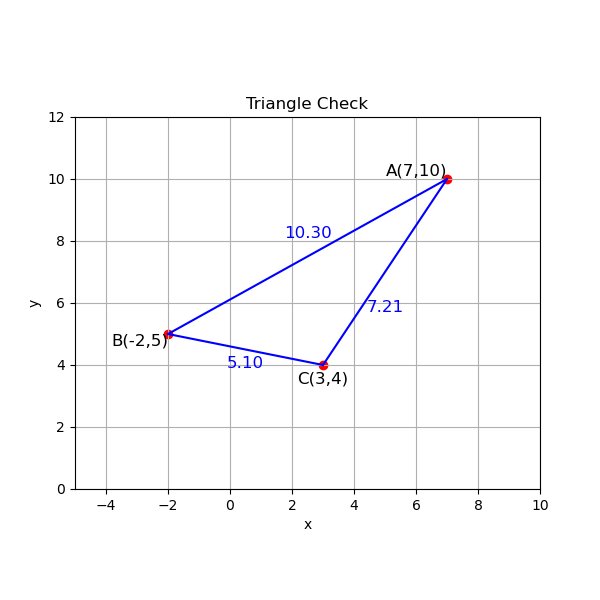
\includegraphics[width=0.5\linewidth]{figs/01.png}
   \caption{Plot of $\triangle$ABC}
   \label{Plot_1}
\end{figure}
\end{frame}

 % --------- CODE APPENDIX ---------
\section*{Appendix: Code}

% C program
\begin{frame}[fragile]{File: points.c}
\begin{lstlisting}[language=C]
#include <stdio.h>

int main() {
  FILE *fp;

  // -------------------
  // Question 2.5.32
  // -------------------


  fp = fopen("points.dat", "w");
  fprintf(fp, "%d,%d,%d\n", 7, 10, 0);  // A
  fprintf(fp, "%d,%d,%d\n", -2, 5, 0);   // B
  fprintf(fp, "%d,%d,%d\n", 3, 4, 0); // C
  fclose(fp);
  return 0;
  }
\end{lstlisting}
\end{frame}

% Python calling C
\begin{frame}[fragile]{File: call\_c.py}
\begin{lstlisting}[language=Python]
import subprocess

# Compile the C program
subprocess.run(["gcc", "points.c", "-o", "points"])

# Run the compiled C program
result = subprocess.run(["./points"], capture_output=True, text=True)

# Print the output from the C program
print(result.stdout)
\end{lstlisting}
\end{frame}

% Python plotting
\begin{frame}[fragile]{File: plot.py}
\begin{lstlisting}[language=Python]
import matplotlib.pyplot as plt
import numpy as np

# Points A(7,10), B(-2,5), C(3,4)
A = np.array([7, 10])
B = np.array([-2, 5])
C = np.array([3, 4])

# Function to calculate distance between two points
def distance(p1, p2):
    return np.sqrt((p2[0] - p1[0])**2 + (p2[1] - p1[1])**2)

# Calculate distances
AB = distance(A, B)
BC = distance(B, C)
CA = distance(C, A)

# Plotting the triangle
plt.figure(figsize=(6, 6))
plt.plot([A[0], B[0]], [A[1], B[1]], 'b-', label="AB")
plt.plot([B[0], C[0]], [B[1], C[1]], 'b-', label="BC")
plt.plot([C[0], A[0]], [C[1], A[1]], 'b-', label="CA")

# Annotating points
plt.text(A[0], A[1], 'A(7,10)', fontsize=12, ha='right', va='bottom')
plt.text(B[0], B[1], 'B(-2,5)', fontsize=12, ha='right', va='top')
plt.text(C[0], C[1] - 0.2, 'C(3,4)', fontsize=12, ha='center', va='top')

# Highlighting the vertices
plt.scatter([A[0], B[0], C[0]], [A[1], B[1], C[1]], color='red')
\end{lstlisting}
\end{frame}

\begin{frame}[fragile]{File: plot.py}
\begin{lstlisting}[language=Python]
# Displaying distances on the plot with offset adjustments
mid_AB = (A + B) / 2
mid_BC = (B + C) / 2
mid_CA = (C + A) / 2

# Adjusting text placement for better spacing
plt.text(mid_AB[0], mid_AB[1] + 0.6, f'{AB:.2f}', fontsize=12, color='blue', ha='center')
plt.text(mid_BC[0], mid_BC[1] - 0.6, f'{BC:.2f}', fontsize=12, color='blue', ha='center')
plt.text(mid_CA[0], mid_CA[1] - 1.3, f'{CA:.2f}', fontsize=12, color='blue', ha='center')

# Setting plot limits and labels
plt.xlim(-5, 10)
plt.ylim(0, 12)
plt.gca().set_aspect('equal', adjustable='box')
plt.xlabel('x')
plt.ylabel('y')
plt.title('Triangle Check')

# Show the plot
plt.grid(True)
plt.show()
\end{lstlisting}
\end{frame}

\end{document}
